%% Submissions for peer-review must enable line-numbering 
%% using the lineno option in the \documentclass command.
%%
%% Preprints and camera-ready submissions do not need 
%% line numbers, and should have this option removed.
%%
%% Please note that the line numbering option requires
%% version 1.1 or newer of the wlpeerj.cls file, and
%% the corresponding author info requires v1.2

\documentclass[fleqn,10pt,lineno]{wlpeerj} % for journal submissions
% \documentclass[fleqn,10pt]{wlpeerj} % for preprint submissions

\usepackage{hyperref}
\usepackage{minted}
\usepackage{subcaption}
\usepackage{multirow}
\usepackage{a4wide}

% for track changes. See https://tex.stackexchange.com/questions/65453/track-changes-in-latex
\usepackage{changes}
\definechangesauthor[name={Egon}, color=blue]{ew}
\definechangesauthor[name={Lars}, color=teal]{lw}
%\setremarkmarkup{(#2)}

\title{Citation.js: A Decentralised, Modular Bibliography Tool in JavaScript}

\author[1]{Lars Willighagen}
\affil[1]{Eindhoven, The Netherlands}
\corrauthor[1]{Lars Willighagen}{lars.willighagen@gmail.com}

% \keywords{Keyword1, Keyword2, Keyword3}

\begin{abstract}

\end{abstract}

\begin{document}

\flushbottom
\maketitle
\thispagestyle{empty}

\section*{Introduction}

With the goal of scientific publishing being the distribution of knowledge, it is important that this knowledge is actually distributed properly, which includes the accessibility and findability of these publications. One way findability has improved in the last few decades, is the transition from text-based citations to the use of Persistent IDentifiers (PIDs), Digital Object Identifiers (DOIs) being the most common. These PIDs are then linked to central stores of machine-readable bibliographic information.

However, there are lots of different stores, most with their own formats. On top of that, most citation managers, like Mendeley (www.mendeley.com), EndNote, Zotero (www.zotero.org) and even Office Word, have own formats as well \added[id=ew, remark={Add references where people can read (and verify!) about those internal formats, or explain in this paragraph (and then likely still need references). The REF can be a review paper or so...}]{REF}. Because of that, citation managers have to maintain parsers for most of those formats. Citation.js brings this functionality to most platforms by using JavaScript, allowing developers to have full control of the machine the software is running on.

To still ensure performance on the client machine, or the web page if the program is running in the browser, Citation.js is fully modularised. Formats are bundled in thematic plugins, which can be installed separately. This can be seen as a regression with respect to for example Zotero; the plugins \textit{have} to be installed separately. However, it is a necessary choice, especially if Citation.js is to be used on anything other then dedicated sites.


\section*{Methods}

\subsection*{Software Development}

The software was developed using modern standards. This included: version control with Git, semantic versioning for releases~\citep{preston-werner_semantic_2013}, open source archives on GitHub and Zenodo, Browserify \citep{noauthor_browserify:_2018} and Babel \citep{noauthor_babel:_2018} builds automated with npm script hooks, integration testing on a CI using the Travis-CI service~\citep{noauthor_travis_2018}, code linting with ESLint~\citep{noauthor_eslint:_2018} and Standard~\citep{noauthor_standard:_2018}, checking \texttt{RegExp}'es for ReDOS vulnerabilities with \texttt{vuln-regex-detector}~\citep{davis_impact_2018}, and API documentation with JSDoc~\citep{noauthor_jsdoc:_2018}.

The development process took place with node and npm. First off, any changes would be linted and tested with the available tools. Bugs or new features can also warrant the introduction of new test cases. If the changes work properly, they are then commited into the version control. If the changes warrant a new release, or if enough changes have piled up for a new release, the change log is updated. Updating the version in the package metadata automatically triggers the linters and test runners, preventing accidental mistakes. Afterwards, publishing the package to npm automatically generates files necessary for the package.

\subsection*{Libraries and others}

Apart from tools used for development, Citation.js also uses a number of runtime libraries. Their function and the reason for using them is explained below.

\begin{description}
\item[\texttt{@babel/polyfill}]
is a runtime library which fills in support for modern APIs on older platforms. It comes with the use of Babel to transform modern syntax for older platforms.

\item[\texttt{citeproc-js}]
is the official CSL formatting library in JavaScript~\citep{noauthor_csl_nodate}.

\item[\texttt{commander}]
is a utility library, only used for the CLI. It parses the command line arguments and generates documentation.

\item[\texttt{isomorphic-fetch}]
is a specific polyfill for the \href{https://developer.mozilla.org/en-US/docs/Web/API/Fetch_API}{Fetch API}, a modern way of requesting web resources. It works in both node and browsers.

\item[\texttt{sync-request}]
is a way to request web resources synchronously. While performing such operations synchronously is advised against in JavaScript, it is still useful for non-production scientific scripts, and demos.

\item[\texttt{wikidata-sdk}]
is a utility library for working with the Wikidata API.
\end{description}

\section*{Results}

\subsection*{Implementation}

Citation.js employs a number of ways to achieve a balance between function and ease of use. The program consists of three major parts: the bibliography interface, code handling input parsing, and code handling output formatting. The bibliography interface itself is quite simple; it mainly acts as a wrapper around the parsing and formatting parts. These two parts behave in a modularised way, with a common plugin system.

\subsubsection*{Input parsing}

Input parsing works by registered input formats. These registrations include an optional type recognizer and a synchronous and/or an asynchronous transforming the input into a format closer to the final format: CSL-JSON. The new input can then be tested again, and will be parsed iteratively until the final format is reached. Plugin authors are encouraged to create input parsers with as small steps as possible, to allow users to input a variety of different formats.

Type recognition is done with a search tree. First of all, types are ordered by the data type of the input. This is one of: String (unparsed text, identifiers, etc.), SimpleObject (standard JavaScript Object: parsed data, JSON-LD), Array (a possibly non-uniform list of inputs), ComplexObject (other non-literal values) and Primitive (numbers, null, undefined). The data type can be inferred from other format specifications in some cases. Types can also be specified to be a more specific version of something else. For example, a DOI URL is also a normal URL, but should be parsed differently, namely with content negotiation.

Types can then provide a list of predicates, testing if input belongs to that format. To avoid code repetition and make plugin registration code easier to read, certain common tasks can also be accomplished using shortcuts. These shortcuts include testing text against a RegExp pattern, checking for certain properties and checking for the value of elements in an array. These properties can also eliminate the need for an explicit data type: for example, if a RegExp is provided, input can be expected to be a String.

\subsubsection*{Output formatting}

Output formatting is less complicated. Users and developers only have to provide the formatter identifier. Further customization can then be done by providing options, which are automatically forwarded to the formatter. This allows the CSL plugin to take in options specifying the template and locale, for example.

\subsubsection*{Plugin system}

Apart from being able to add input and output formats and schemes on their own, it is also possible to add them in a thematically linked plugin. For example, a BibTeX plugin might consist of a parser for \texttt{.bib} files, a parser for the resulting BibTeX-schemed JSON, and a output formatter to create BibTeX from other sources as well. This plugin could then be combined with, for example, a Bib.TXT plugin, producing a JavaScript package or module, which could be published in package managers like NPM. Code for this plugin would like Fig. \ref{code:plugin}.

For configuring plugins there is also a \texttt{config} option. As an example a \texttt{labelForm} option is added, which could control the way the BibTeX output formatter generates labels. Users of this plugin can then retrieve and modify this configuration. It is also possible to offer internal functions this way, for more fine-grained control.

\begin{figure}[ht]
\centering
\begin{minted}[linenos]{javascript}
let Cite = require('citation-js')

Cite.plugins.add('bibtex', {
  input: {
    '@bibtex/text': {
      parseType: { ... },
      parse (text) { ... }
    },
    '@bibtex/object': {
      parseType: { ... },
      parse (text) { ... }
    }
  },

  output: {
    bibtex (data, options) {
  ...
    }
  },

  config: {
    labelForm: ['author', 'title', 'issued']
  }
})

let bibtexConfig = Cite.plugins.config.get('bibtex')
bibtexConfig.labelForm = ['author', 'issued', 'year-suffix']
\end{minted}
\caption{\textbf{Possible structure of a plugin for BibTeX.}
In this example package, line 1 loads Citation.js and lines 2-24 adds the plugin. This plugin consists of two input formats (4-13), one output format (15-19) and configuration options (21-23). Some code is omitted for the sake of clarity, and is replaced with ellipsis (\texttt{...}). Lines 26-27 show how this configuration would be used.
}
\label{code:plugin}
\end{figure}

\subsubsection*{Bibliography interface}

The methods for parsing input and formatting output are also included in a general class, \texttt{Cite}. Class instances also have access to opt-in version control (changes are tracked if an explicit flag is passed) and sorting. The latter currently doesn't have effect on CSL bibliographies, as the styles there provide their own sorting method.

\subsubsection*{Supported formats}

Table \ref{table:support} shows the formats supported by Citation.js at the moment.

\begin{table}[ht]
\caption{\textbf{Input and output format support.}
This table only shows general support. For example, the "Wikidata" format is both used for Wikidata identifiers and Wikidata API results.}
\label{table:support}
\begin{tabular}{|l|c|c|}
\hline
\textbf{Format} & \textbf{Input} & \textbf{Output} \\ \hline
BibJSON         & x              &                 \\ \hline
BibTeX          & x              & x               \\ \hline
Bib.TXT         & x              & x               \\ \hline
CSL             & (JSON)   & x               \\ \hline
DOI             & x              &                 \\ \hline
RIS             &                & x               \\ \hline
Wikidata        & x              &                 \\ \hline
\end{tabular}
\end{table}

\subsection*{Distribution}

\subsubsection*{Browser use}

For in-browser use, there is also a standalone JavaScript file available. This includes dependencies. This bundle is built automatically when publishing, and is available through a number of Content Delivery Networks (CDNs) that automatically distribute NPM packages. The \texttt{Cite} class can then be imported and used just as the NPM package, barring browser limitations.

For simple use cases, like inserting static bibliographies, a separate tool was developed, called \texttt{citation.js-replacer}. When included on a page, this replaces every HTML element matching a certain selector, with a bibliography. Figure \ref{code:use} shows an example of another use case. For example, the basic use can be extended to add additional information to references, such as an Altmetric.com score icon or Dimensions citation count.

\begin{figure}[bt!]
\centering
\begin{tiny}
\begin{minted}[linenos,breaklines]{html}
<html>
<head>
  <script src="https://d1bxh8uas1mnw7.cloudfront.net/assets/embed.js"></script>
  <script src="https://cdn.jsdelivr.net/npm/citation-js"></script>
</head>
<body>
  <div id="element"></div>
  <script>
    window.onload = async function () {
      let Cite = require('citation-js')
      let cite = await Cite.async('10.1371/journal.pone.0185809')
      
      let bibliography = cite.format('bibliography', {
        format: 'html',
        append ({DOI}) {
          return ` <span class="altmetric-embed" data-badge-type="badge" data-doi="${DOI}"></span>`
        }
      })
    
      let element = document.getElementById('element')
      element.innerHTML = bibliography
      _altmetric_embed_init()
    }
  </script>
</body>
</html>
\end{minted}
\end{tiny}
\caption{\textbf{Basic use, including appending data to formatted bibliography entries.}
Here, line 4 loads the library, line 10 imports \texttt{Cite}, and line 11 creates an interface for a bibliography with one entry, with metadata from a DOI. Lines 13-18 render the bibliography, with line 14 setting the output to HTML and lines 15-17 appending an Altmetric widget to the entry. Lines 20-21 show the output on the page. Lines 9 and 22 are to avoid race conditions in DOM access. Line 3 and 22 initialize the Altmetric badge.
}
\label{code:use}
\end{figure}

\begin{figure}[ht]
\centering
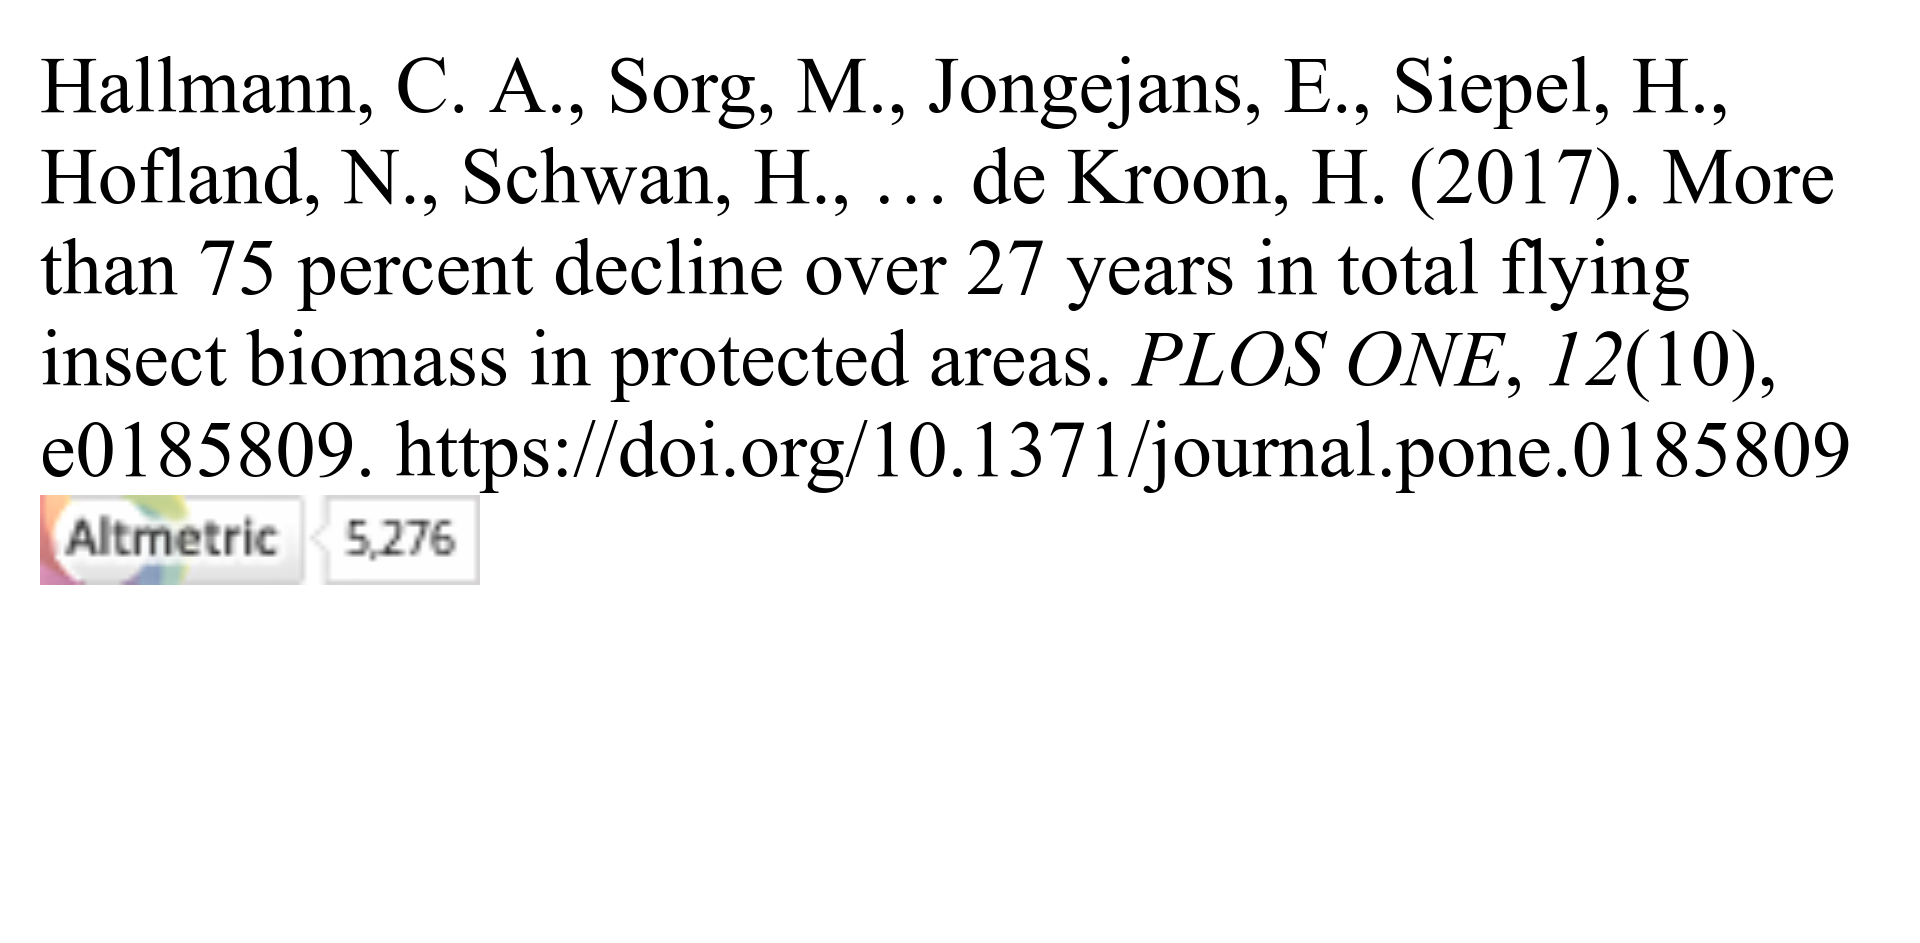
\includegraphics[width=\linewidth]{figures/use_altmetric.png}
\caption{\textbf{Result of the code in Fig. \ref{code:use}.} Note the Altmetric badge at the end.}
\label{fig:use}
\end{figure}

\subsubsection*{NPM package}

Citation.js is published as an npm package on the main npm registry, as \href{https://npm.im/citation-js}{\texttt{citation-js}}. Use of the package is the same anywhere, apart from platform limitations. For example, synchronous requests for web resources, to get metadata for DOIs, is limited on Chrome~\citep{willighagen_make_2017}. Also, the node platform, not being a browser, doesn't have access to the Document Object Model (DOM), and so can't easily use HTML elements as input or output.

Use cases for the npm package include using it when generating content (either at runtime or for static websites) like \href{https://www.pubpub.org/}{PubPub}, and setting up APIs~\citep{willighagen_citation.js:_2017}. It is also useful for converting metadata when text mining. For example, BibJSON is one of the input formats, and can then be converted to BibTeX or formatted.

\subsubsection*{CLI use}

Simple one-time conversions, with no extensive customization, can also be done with Command Line Interface (CLI). Figure \ref{code:cli} shows an example on how to use it. For instance, a list of DOIs can be converted into a single BibTeX file for further use.

\begin{figure}[ht]
\centering
\begin{minted}[breaklines]{bash}
$ npm install --global citation-js

$ citation-js -i dois.txt -t string -s bibtex > dois.bib
\end{minted}
\caption{\textbf{CLI use.}
The first command installs the \texttt{citation-js} command, and may require root privileges. Alternatively, this step can be skipped, and additional commands should be run as \texttt{npx citation-js ...} instead. The second command shows how to convert a list of DOIs from a file (\texttt{-i dois.txt}) can be converted into a non-formatted (\texttt{-t string}) BibTeX (\texttt{-s bibtex}) file. The resulting file is then printed on standard out and redirected into a file (\texttt{> dois.bib}), with additional logging on standard error.
}
\label{code:cli}
\end{figure}

\subsubsection*{Integrations}

The Citation.js npm package can also be used as a library to create integrations with for example word processing systems. For example, \href{https://github.com/RelaxedJS/ReLaXed}{ReLaXed} integrates Citation.js into the Pug templating language to generate citations when creating PDF documents, and \href{https://github.com/larsgw/citation.js-showdown}{a plugin for Showdown} introduces syntax for citations in markdown.

\subsection*{Performance}

The performance of the Citation.js package has been analyzed on a number of different platforms. A common theme is that in browsers, compiling the script and importing the library takes about 120 ms, compiling itself being a little less than half of that. Node.js on the other hand takes about 1 s to initialize, both when the source consisting of multiple files is imported, and when a bundle is imported. This is possibly because Chrome caches compiled JavaScript reducing the compiling times from around 50 ms to about 8 ms.

The results were obtained with the default settings for each of the platforms. In Chrome, this was achieved by using guest mode, while Node and Firefox were not configured to begin with.

As shown in Fig. \ref{fig:perf} and Table \ref{table:size}, time taken to import the library mainly consists of importing \texttt{@babel/polyfill}. This is because adding the polyfills requires repeated feature detection. After that the actual code is imported in two parts. In the first part, where core functionality like the Cite interface is loaded, the main culprit is \texttt{addTypeParser}, with 0.13 ms per call on average. In the second part, loading output-related code, importing \texttt{citeproc-js} takes the longest with a single call of 2.82 ms.
Note that that Firefox uses Just-In-Time compilation (JIT), compiling pieces of code when they are used a lot.

\begin{figure}[bt!]
\begin{subfigure}{1.1\textwidth}
  \centering
  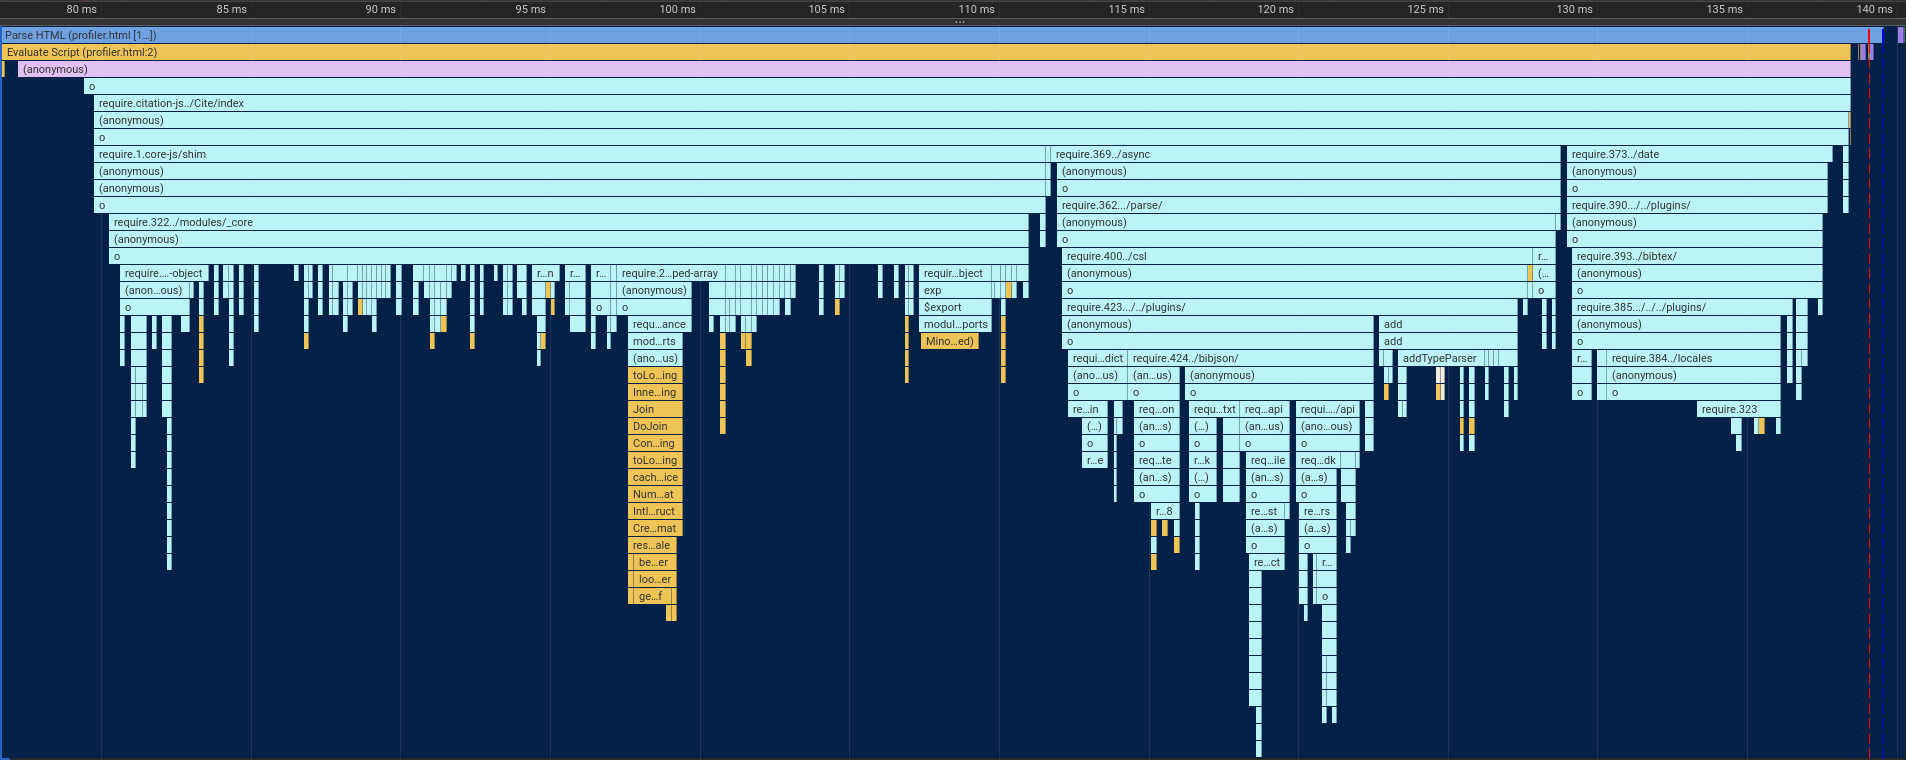
\includegraphics[width=\linewidth]{figures/perf_chrome.png}
\caption{\textbf{Chrome 71}}
  \label{fig:perf-chrome}
\end{subfigure}
\begin{subfigure}{1.1\textwidth}
  \centering
  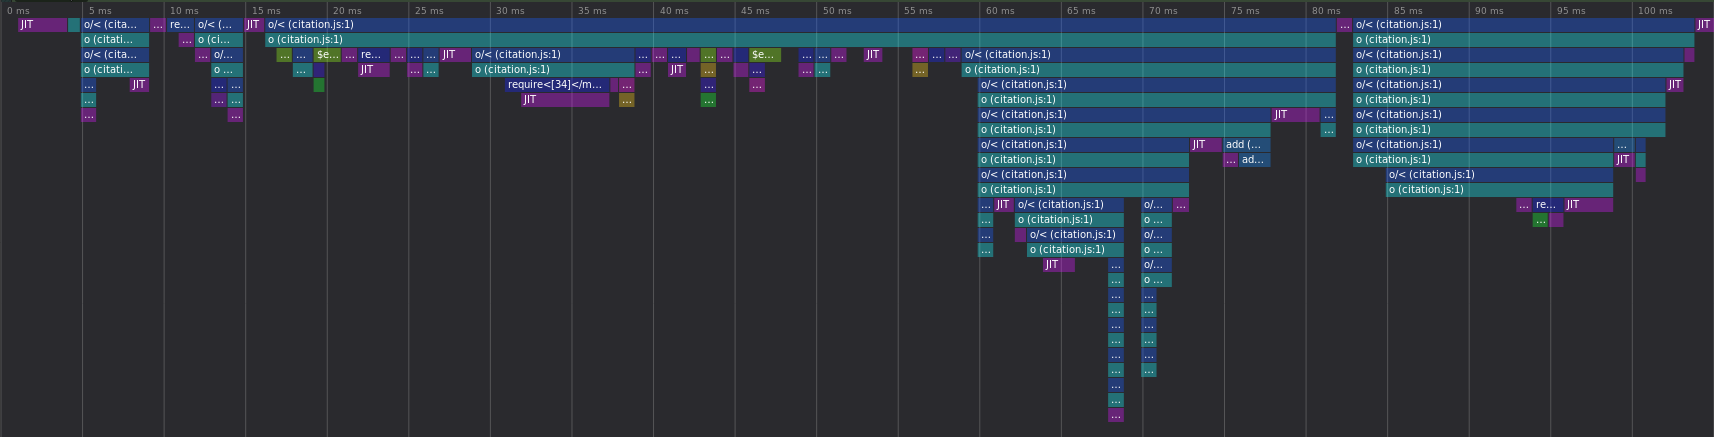
\includegraphics[width=\linewidth]{figures/perf_ff.png}
  \caption{\textbf{Firefox 64}}
  \label{fig:perf-ff}
\end{subfigure}
\caption{\textbf{Initialization performance results on different platforms.}
Actual timings may very depending on the device, OS and cache. Note that Chrome starts with 40 ms of compiling time that is cached on subsequent runs. Firefox compiles JIT (Just-In-Time), while the code is running. Both graphs show three parts, one loading polyfills from \texttt{@babel/polyfill} taking up half the loading time, followed by two parts mainly loading input parsing and output formatting code respectively. Profiling data is available in supplemental information.}
\label{fig:perf}
\end{figure}

While code execution is one part, one should also look into the file size. This is especially important in the browser, which has to fetch the library when loading the page.

\begin{table}[ht]
\caption{\textbf{Browser bundle breakdown.} Running time is the approximate time it takes to import the script with browserify \texttt{require} in the Chrome data set. Note that a big part of the \texttt{plugin-csl} "own" code is serialized styles and locales from the CSL repository. Minified and g-zipped, the code is just 177 kb.}
\label{table:size}
\begin{tabular}{|l|l|r|r|r|r|}
\hline
\multicolumn{2}{|c|}{\multirow{2}{*}{\textbf{Part}}} & \multicolumn{3}{c|}{\textbf{Size}}                                                                                   & \multicolumn{1}{c|}{\multirow{2}{*}{\textbf{Running time}}} \\ \cline{3-5}
\multicolumn{2}{|c|}{}                               & \multicolumn{1}{c|}{\textbf{Own}} & \multicolumn{1}{c|}{\textbf{Dependencies}} & \multicolumn{1}{c|}{\textbf{Total}} & \multicolumn{1}{c|}{}                                       \\ \hline
\multirow{10}{*}{Citation.js}    & Backport          & 5.9 kb                            & -                                          & 5.9 kb                              & 5.9 ms                                                      \\ \cline{2-6} 
                                 & core              & 99.7 kb                           & 33.9 kb                                    & 133.5 kb                            & 8.3 ms                                                      \\ \cline{2-6} 
                                 & plugin-bibjson    & 7.6 kb                            & -                                          & 7.6 kb                              & 3.5 ms                                                      \\ \cline{2-6} 
                                 & plugin-bibtex     & 42.9 kb                           & -                                          & 42.9 kb                             & 2.6 ms                                                      \\ \cline{2-6} 
                                 & plugin-csl        & 87.0 kb                           & 461.8 kb                                   & 548.9 kb                            & 3.2 ms                                                      \\ \cline{2-6} 
                                 & plugin-doi        & 6.6 kb                            & -                                          & 6.6 kb                              & 0.6 ms                                                      \\ \cline{2-6} 
                                 & plugin-ris        & 11.1 kb                           & -                                          & 11.1 kb                             & 0.5 ms                                                      \\ \cline{2-6} 
                                 & plugin-wikidata   & 22.1 kb                           & 40.4 kb                                    & 62.4 kb                             & 2.2 ms                                                      \\ \cline{2-6} 
                                 & name              & 16.6 kb                           & -                                          & 16.6 kb                             & 1.1 ms                                                      \\ \cline{2-6} 
                                 & date              & 7.3 kb                            & -                                          & 7.3 kb                              & 0.2 ms                                                      \\ \hline
\multirow{2}{*}{Additional}      & @babel/polyfill   & -                                 & 197.3 kb                                   & 197.3 kb                            & 32.0 ms                                                     \\ \cline{2-6} 
                                 & Browserify        & -                                 & 6.8 kb                                     & 6.8 kb                              & 0.2 ms                                                      \\ \hline
\multicolumn{2}{|l|}{Total}                          & 306.8 kb                          & 740.1 kb                                   & 1046.8 kb                           & 60.3 ms                                                     \\ \hline
\end{tabular}
\end{table}

\section*{Discussion}

\subsection*{Use of formal grammars for parsing}

Apart from more common formats like JSON, XML and YAML, Citation.js has to parse a number of text formats with syntax specific to that format, like BibTeX and RIS. While one can use standard or even built-in parsers for common formats, that is usually not possible for the latter formats.

To solve this, one can employ formal grammars, which can be translated into code parsing and validating input. Examples of libraries working with grammars are PEG.js and nearley.js. Creating grammars has the benefits of not having to write and maintain code validating and parsing input, and having a readable grammar instead of a complex program file.

However, there are also drawbacks. Generating these grammars requires an extra build step, which in the case of Citation.js cannot be integrated with a similar step due to a lack of tooling. On top of that, generated code usually has poor performance or large size, and in the case of nearley.js uses a runtime library.

Because of that it may be preferable to write custom parsers in some cases. Take RIS, which has no balanced brackets or quotes, and doesn't need much more than simply iterating over the individual lines.

\subsection*{Converting between formats and standardized crosswalks with linked data}

Converting input data like parsed BibTeX, BibJSON or Wikidata API results into another format and back can get very repetitive in terms of code. Yet, there are still cases where special handling is needed. Since different formats call for different needs, each plugin has developed its own system to deal with this. Unifying this into a single, performant, reusable and developer-friendly system would be preferable.

To convert one data format (or scheme) to another, a number of different things must be done. First of all, for most properties a simple mapping suffices: \texttt{title} in BibTeX refers to the same concept as it does in BibJSON and CSL-JSON. On top of that, the property coincides with \texttt{TI} in RIS. This mapping could come in the form of a JSON-LD context, as done by CodeMeta.

Second, the data format needs to be converted. While \texttt{title} in BibTeX can have formatting in the form of \TeX, \texttt{title} in CSL-JSON uses a subset of HTML for formatting, and \texttt{TI} in RIS doesn't have formatting at all. Properties can also have different data types. In CSL-JSON, \texttt{author} is a list of objects, while \texttt{authors} in BibTeX, which describes the same concept, is serialized text delimited by " and ". Both of these examples could be handled by defining two converters for each pair of formats, one for converting from A to B and one for converting back. It would also be possible to convert every format to a central format C, and convert C to every format. This is what Citation.js currently does. It is however important that format C can hold as much information as could be represented in any other format, as to prevent information loss when converting between two formats that have a certain property via a central format that doesn't have that property.

Third, there might not be a one-to-one mapping between properties. For instance, \texttt{pages} in CSL-JSON maps to both \texttt{start} and \texttt{end} in CFF. Alternatively, \texttt{pages}, \texttt{issue}, \texttt{volume} and \texttt{ISSN} are all top-level properties in CSL-JSON, while the corresponding properties in Wikidata are proposed to be nested in the journal property. If the nested values are deserialized, this could be expressed in JSON-LD contexts. However, in the first example it cannot, since JSON-LD cannot distinguish between parts of strings.

Lastly, some mappings are context-dependent. For example, consider the CSL-JSON properties \texttt{author} and \texttt{reviewed-author} in relation to the RIS properties author (\texttt{AU}) and reviewer (usually \texttt{C4}). In normal entries, \texttt{AU} maps to \texttt{author}. However, if the entry being converted is a review, \texttt{AU} maps to \texttt{reviewed-author} while \texttt{author} maps to \texttt{C4}.

In conclusion, a number of different things need to be taken into account when writing a system for crosswalks. While a JSON-LD context would scale very well without a central format, most cases restrict the usefulness. Alternatively, a custom system could be developed that defines as much mapping as possible to and from a central format, with special cases for the third and last restrictions. Additional mappings to common formats, to cover properties missing from the central format could be added, with caution not to create critical dependencies on other formats. Or, given the complexity of the systems, it may be best to create for each format, allowing optimization for the special cases of that format.

\subsection*{Use of GraphQL for API queries}

With REST APIs comes the problem of over-fetching and under-fetching. This means that when fetching a resource it may contain too much unneeded information, require additional calls to the API, or both. This causes unnecessary load on both the client and the server, as both have to process more calls with more network bandwidth.

Using GraphQL APIs circumvents this problem by allowing the client to specify exactly what data it needs. However, not all endpoints may have a GraphQL API available, so this solution cannot be used reliably. Another drawback is that the GraphQL schema used for the API can impose limits, like pagination and some data simply not being available.

\subsection*{Further modularisation}

While the different plugins operate mostly independently now, they are still part of the bundle, slowing down the code unnecessarily in many use cases. It is possible to strip these plugins and publish them under a different name, like \texttt{@citation-js/plugin-software-formats}. To ensure compatibility, the 'classic' selection of plugins that are built-in right now could be published under \texttt{citation-js} functioning as it does right now, and a bare repository allowing for more customization could be published under \texttt{@citation-js/core}.

\subsection*{Support for additional formats}

Apart from the formats currently supported in Citation.js, there are plans to include more formats. These will be published in thematic plugins. For example, formats used to describe software projects are joined in the plugin \texttt{@citation-js/plugin-software-formats}. These formats will also include linked data scraped from web pages.

\subsection*{Scraping from source versus fetching from central stores}

When getting data from for example the Wikidata API or scraped from a web page, that data might be incomplete. However, if part of the data you get is the DOI linked to the entity queried, you could amend that data with data fetched from a central store like Crossref or DataCite. However, due to difficulties with prioritizing data sources and non-trivial merging conflicts this has not yet been implemented.

\section*{Acknowledgments}

\added[id=ew]{Here you can thank people who use it and/or gave feedback.}

\bibliography{citations}

\end{document}